\documentclass[a4paper,12pt]{article}
\usepackage[T1]{fontenc}
\usepackage{rotating}
\usepackage{lscape}
\usepackage{amssymb,amsmath,amssymb}
\usepackage[stable]{footmisc}
\usepackage{lmodern}
\usepackage{libertine}
\usepackage[libertine]{newtxmath}
\usepackage[scale=0.825]{FiraMono}
\usepackage[authoryear]{natbib}
\usepackage{babelbib}
\usepackage{booktabs, makecell, longtable}
\usepackage[usenames,dvipsnames]{xcolor}
\definecolor{darkblue}{rgb}{0.0,0.0,0.55}
\setcitestyle{aysep={}} 
\usepackage{etoolbox}
\makeatletter
\patchcmd{\NAT@citex}
  {\@citea\NAT@hyper@{%
	 \NAT@nmfmt{\NAT@nm}%
	 \hyper@natlinkbreak{\NAT@aysep\NAT@spacechar}{\@citeb\@extra@b@citeb}%
	 \NAT@date}}
  {\@citea\NAT@nmfmt{\NAT@nm}%
   \NAT@aysep\NAT@spacechar\NAT@hyper@{\NAT@date}}{}{}
\patchcmd{\NAT@citex}
  {\@citea\NAT@hyper@{%
	 \NAT@nmfmt{\NAT@nm}%
	 \hyper@natlinkbreak{\NAT@spacechar\NAT@@open\if*#1*\else#1\NAT@spacechar\fi}%
   {\@citeb\@extra@b@citeb}%
	 \NAT@date}}
  {\@citea\NAT@nmfmt{\NAT@nm}%
   \NAT@spacechar\NAT@@open\if*#1*\else#1\NAT@spacechar\fi\NAT@hyper@{\NAT@date}}
  {}{}
\makeatother
\usepackage{setspace}
\usepackage[top=2cm,bottom=2cm,left=2cm,right=2cm]{geometry}
\usepackage{hyperref}
\usepackage{graphicx}
\usepackage{dcolumn}
\usepackage{float}
\floatplacement{figure}{H}
\usepackage{pgf}
\usepackage{tikz}
\usetikzlibrary{arrows}
\usetikzlibrary{positioning}
\usepackage{mathtools}
\usepackage{caption}
\usepackage[UKenglish]{babel}
\usepackage[UKenglish]{isodate}
\cleanlookdateon
\exhyphenpenalty=1000
\hyphenpenalty=1000
\widowpenalty=10000
\clubpenalty=1000
\onehalfspacing
%\urlstyle{same}  % don't use monospace font for urls

\hypersetup{pdftitle={Article Title},
	pdfauthor={Your Name},
	pdfsubject={Subject},
    pdfkeywords={A, B, C},
	pdfborder={0 0 0},
	breaklinks=true,
	linkcolor=Mahogany,
	citecolor=Mahogany,
	urlcolor=darkblue,
	colorlinks=true}

\doublespacing

\title{\textbf{Article Title}}

\author{Author Name\thanks{Academic position, Department of Cool Sciences, Some University, professional address,  \href{mailto:your.email@univesity.com}{\texttt{your.email@university.edu}},  \href{http://website.com}{\texttt{http://website.com}}. I would like to thank \dots}
}

\date{\today}

\begin{document}
\maketitle

\begin{abstract}
 \noindent
 Lorem ipsum dolor sit amet, consectetur adipiscing elit. Ut vitae porttitor metus, eu congue erat. Nam hendrerit luctus purus vel feugiat. Pellentesque et nunc tellus. Curabitur iaculis interdum commodo. Aenean rhoncus ipsum ante, id hendrerit turpis sodales ut. Quisque ultricies interdum neque, id mattis tellus mattis et. Nam feugiat dui eros, sit amet malesuada elit iaculis ut. Donec placerat metus ac lacus ultricies posuere. Maecenas imperdiet ut magna id tincidunt. Nulla in leo pulvinar, ultricies purus at, condimentum nisl. Nulla facilisi.

 \vspace{.5cm}
 \noindent
 \textbf{Keywords}: A, B, C, D, E

 \vspace{.25cm}
 \noindent
 \textbf{JEL Classification Codes}: A00, B11, C22
\end{abstract}

\newpage

\section{Introduction}
\label{sec:intro}

Regular, \textit{italics}, \textbf{boldface}, \texttt{monospaced}.\footnote{This is a footnote. A citation: \citet{chazkel2011laws}. A website: \href{http://danilofreire.com}{\texttt{http://danilofreire.com}}.} Lorem ipsum dolor sit amet, consectetur adipiscing elit. Ut vitae porttitor metus, eu congue erat. Nam hendrerit luctus purus vel feugiat. Pellentesque et nunc tellus. Curabitur iaculis interdum commodo. Aenean rhoncus ipsum ante, id hendrerit turpis sodales ut. Quisque ultricies interdum neque, id mattis tellus mattis et. Nam feugiat dui eros, sit amet malesuada elit iaculis ut. Donec placerat metus ac lacus ultricies posuere. Maecenas imperdiet ut magna id tincidunt. Nulla in leo pulvinar, ultricies purus at, condimentum nisl. Nulla facilisi.

Curabitur facilisis metus non ex interdum elementum. Maecenas suscipit massa nec lacus placerat lacinia. Mauris eu ex consequat magna mollis mollis et quis turpis. Maecenas consequat nisi eget venenatis laoreet. Donec egestas at tortor commodo dapibus. Sed blandit vehicula semper. Sed ex dolor, sollicitudin id vehicula et, egestas a elit. Nullam in volutpat purus. Sed sed nibh porta nulla varius sodales vitae sed magna. Pellentesque eu ligula quis felis posuere finibus non sed velit. Nunc a elementum ante. Ut fermentum, ante nec accumsan dapibus, velit mi rhoncus metus, a feugiat ipsum metus vitae justo. Phasellus non metus at justo varius varius. 

\begin{figure}[!htbp]
 \centering
 \begin{minipage}[b]{0.45\textwidth}
  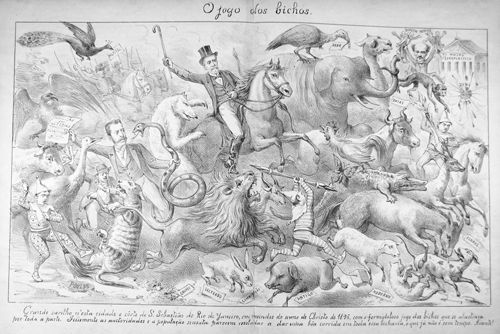
\includegraphics[width=\textwidth, height=6cm]{images/bicho01.jpg}
 \end{minipage}
 \hfill
 \begin{minipage}[b]{0.45\textwidth}
  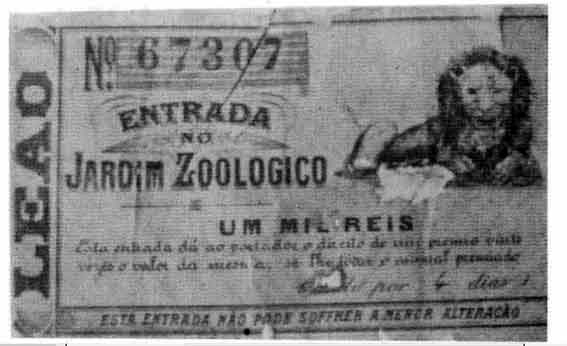
\includegraphics[width=\textwidth, height=6cm]{images/bicho02.jpg}
 \end{minipage}
 \caption{Left: cartoon of the Baron of Drummond and the animals of the \emph{jogo do bicho} (1896). Right: entry ticket to Rio's Zoological Garden that allowed the bearer to join the raffle. Sources: Instituto Histórico e Geográfico Brasileiro, Rio de Janeiro, Revista Illustrada, ano 21, no. 718 (1896) and Museu da Imagem e do Som, Rio de Janeiro.}
 \label{fig:barao}
\end{figure}

\newpage

\subsection{Subsection: Equations}
\label{sub:eq}

\begin{align}
 f(x)  &= a x^2+b x +c   &   g(x)  &= d x^3 \\
 f'(x) &= 2 a x +b       &   g'(x) &= 3 d x^2
\end{align}


\begin{equation}
  u(x) =
  \begin{cases}
   \exp{x} & \text{if } x \geq 0 \\
   1       & \text{if } x < 0
  \end{cases}
\end{equation}

\vspace{.5cm}

\subsubsection{Subsubsection: Table}
\label{subsub:table}

\def\onepc{$^{\ast\ast}$} \def\fivepc{$^{\ast}$}
\def\tenpc{$^{\dag}$}
\def\legend{\multicolumn{4}{l}{\footnotesize{Significance levels
:\hspace{1em} $\dag$ : .1 \hspace{1em}
$\ast$ : .05 \hspace{1em} $\ast\ast$ : .01 \normalsize}}}

\begin{table}[htbp]\centering \footnotesize \caption{Logistic Regressions for Civil War Incidence \label{table1:sumstats}}
\begin{tabular}{l c c c}\hline\hline
\multicolumn{1}{c}{\textbf{Variable}} & \textbf{Model I}
 & \textbf{Model II}& \textbf{Model III}\\ \hline
p\_xrcomp1$_{t-1}$ & $-$0.914**\\
(selection) & (0.184)\\
p\_xrcomp2$_{t-1}$ & $-$2.218**\\
(dual / transition) & (0.391)\\
p\_xrcomp3$_{t-1}$ & $-$0.783**\\
(election) & (0.236)\\
p\_xrcomp\_n$_{t-1}$ & & 0.457\\
(autocratisation) & & (0.440)\\
p\_xrcomp\_p$_{t-1}$ & & & 0.150\\
(democratisation) & & & (0.430)\\
constant & $-$7.599** & $-$6.357** & $-$7.136**\\
\hline
N & 2579 & 2600 & 2819\\
Wald $\chi^2$ & (8) 174.63 & (13) 154.40 & (8) 174.63\\
Log Pseudolikelihood & $-$779.945 & $-$844.045 & $-$916.790\\
Pseudo R$^2$ & 0.115 & 0.100 & 0.102\\
\hline
\legend\\
{\footnotesize Standard errors in parentheses}\\
\hline
\end{tabular}
\end{table}

\newpage
\bibliography{references.bib}
\bibliographystyle{apalike}
\end{document}
